\documentclass[a4paper, oneside]{memoir}

\usepackage[english]{babel} % load typographical rules for the english language
\usepackage{graphics} % for \scalebox
\usepackage{hyperref} % for \href
\usepackage{enumitem} % for options to the enumerate environment
\usepackage[cache=false]{minted} % code inclusion
\usepackage{dirtytalk} % for \say quotation
\usepackage{adjustbox} % for \adjustbox environment

\usepackage{tikz} % for diagrams

% https://github.com/latex3/babel/issues/51
\makeatletter\AtBeginDocument{\let\@elt\relax}\makeatother

% styling
\setsecnumdepth{subsubsection} % how deep to number sections
\setlength{\parindent}{0em} % horizontal indent for first line of paragraph
\setlength{\parskip}{1em} % vertical space between paragraphs

\newcommand{\textdesc}[1]{\textit{\textbf{#1}}}
\newcommand{\descitem}[1]{\item \textdesc{#1}}
\newcommand{\quoted}[1]{\textsl{\say{#1}}}

\title{Report Writing \\ \scalebox{0.85}{for Software BSc and MSc Projects}}
\author{Aslak Johansen}

\begin{document}

\maketitle

\setcounter{tocdepth}{2}
\tableofcontents

%%%%%%%%%%%%%%%%%%%%%%%%%%%%%%%%%%%%%%%%%%%%%%%%%%%%%%%%%%%%%%%%%%%%%%%%%%%%%%%%
%%%%%%%%%%%%%%%%%%%%%%%%%%%%%%%%%%%%%%%%%%%%%%%%%%%%%%%%%%%%%%%%%%% Introduction
\chapter{Introduction}

% purpose

\section{Advisor}

First of all: All advisors are different. If your advisor disagrees with this section, then they are right and this section is wrong.

\subsection{Role}

% inclusion: report structure (when presented with text of reasonable quality)

% exclusion: basic grammar, spelling

\subsection{Interaction}

The perfect interaction model for supervision depends on the specific project. However, as a starting point I like to have a weekly recurring status meeting of 30 minutes that goes into the calendar. That way there is time allocated. If I don't receive an agenda over Discord 24 hours before the meeting I consider it canceled and may reallocate the time. In some weeks there won't be anything to cover in this status meeting, and in other weeks there may be a need for an extra meeting.

When it comes to the day-to-day supervision (aka the small questions and messages) I find that a per-project Discord channels works best. That setup also integrates well with online meetings and screensharing.

\subsection{Choice}

% intro: partnership
The relationship between the students of a group, their advisor(s) is a partnership. Ideally, all partners should get something out of it. From the advisors side that will usually be a domain or field of interest, and the project could be rooted in a research project.

% if it doesnt work out
If you have a negative previous experience with a potential advisor (e.g., from a bachelor project), then you should obviously look elsewhere. Do note that this is does not have to indicate more that incompatibilities of personality types.

% reasons
Good reasons to choose a advisor may include:
\begin{itemize}
  \item You like the advisor on a personal level. Do note that supervision is not a personal relationship.
  \item You have enjoyed classes taught by the advisor. Do note that supervision style may differ from teaching style.
  \item Overlap in technological interests.
  \item Overlap in domain interests.
\end{itemize}

\section{Project Size}
\label{sec:projectsize}

% project length
Currently, at SDU, a BSc project is 15 ECTS points across the spring semester, and a MSc project is either 30 ECTS across the spring semester or 40 ECTS points across two semesters starting in the fall. The workload of the 40 ECTS variant is distributed so that 10 ECTS points are placed in the fall semester and the remaining 30 ECTS points fill up the entire spring semester. When that model is followed, the fall semester is typically spent interviewing stakeholders, doing the literature review and generally laying things out so that everything is ready for a focused spring semester. If you have found a project that gets you excited, and you should, then I really recommend that you choose a 40 ECTS point MSc. The 30 ECTS points variant has a tendency to get crammed. Be aware that there is a deadline for applying for a 40 ECTS project.

\section{Group Composition}

% don't do it alone
Groups of one can work, but they rarely do. What usually happens is that -- lacking experience with a project of this size -- the student starts postponing tasks (e.g., due to waning motivation). Groups of two are much more robust in that sense, likely due to a combination of a feeling of responsibility towards the other group member and the shared support structure. Groups of three can also work, but here the trick becomes (i) to size to project workload, and (ii) to make it clear that all have done their fair share of the project.

% friends but not too good friends
It is important for group members to be on good terms. Positive experience from previous groupwork is a plus. However, groups consisting of too \textsl{good} friends have a tendency to find topics irrelevant to the project to spend their time on. While that is a healthy thing it is not conductive in terms of progressing the project.

\section{Project Choice}

\section{Industrial Collaboration}

% positive

% seen through the eyes of the company

% negative

\subsection{Non-Disclosure Agreement}

% purpose and involvement
Often, an industrial collaborator will insist on the anyone coming into contact with what they consider company secrets to sign a nondisclosure agreement (NDA). That includes the group members and SDU. SDU will sign this on behalf of the advisor(s) and censor. You can get the ball rolling by contacting \href{mailto:contracts@sdu.dk}{contracts@sdu.dk}. But before doing so, you should read their intro\footnote{\url{https://www.sdu.dk/en/om_sdu/institutter_centre/tekinnovation/for_studerende/nda}}.

% warning
You should, however, be aware that getting an NDA in place can be a lengthy process. All parties need to agree on the legalese and that means that representatives of the legal organizations have to dead through the document and agree on the contents. SDU has a standard NDA, but the industrial partner may not be happy about it. Expect this process to be measured in months, and expect not to have access to material from the industrial collaborators before it is in place. If you are doing a 40 ECTS project that is likely to be highly inconvenient, but if you are doing a 30 ECTS project that can quickly become detrimental. The lesson learned is to start as early as possible, and aim to have that NDA in place \textsl{before} handing in the project description.

\section{Deadlines}

At SDU there are a few deadlines to be concerned with. These are:
\begin{itemize}
  \item The deadline for signing up for a 40 ECTS MSc project and is, naturally, only applicable to MSc projects. See section \ref{sec:projectsize} for details.
  \item The deadline of handing in the project description. Please note that this needs to be approved. See section \ref{sec:projectdesc} for details.
  \item Usually (but not always) there is a poster session approx 1 month before handin of the final report. It may be mandatory for you and it may be optional.
  \item The deadline of handing in the final report.
\end{itemize}

%%%%%%%%%%%%%%%%%%%%%%%%%%%%%%%%%%%%%%%%%%%%%%%%%%%%%%%%%%%%%%%%%%%%%%%%%%%%%%%%
%%%%%%%%%%%%%%%%%%%%%%%%%%%%%%%%%%%%%%%%%%%%%%%%%%%%%%%%%%%% Project Description
\chapter{Project Description}
\label{sec:projectdesc}

The project description is a document you hand in via \url{spoc.sdu.dk}. This document frames your project by describing which problem you will be addressing and how you plan on doing so. When writing this, it is important to keep your learning objectives in mind. Through the report you end up writing for this project, it should be clear to censor that you have reached all of your learning objectives.

But lets imagine that you end up with a project description that makes it is impossible for you to do any work that relates to one of the learning objectives. Accordingly, it will be impossible for you to not a have at least one major weakness, and thus you cannot possibly get a higher grade than 7.

The strategy for getting the best possible grade (on the Danish 7-point grading scale) is to focus on doing best in the worst of the learning objectives. This is a direct consequence of the focus on weaknesses. However, all projects are different and not all learning objectives are equally important for all projects. At the end of the day, all learning objectives are in effect, only with weights depending on the concrete project.

\section{Structure}

The structure of the project description is not set in stone. I usually recommend following the following template:

\begin{enumerate}
  \descitem{Context} This section covers all background information necessary for understanding the "Problem" and "Approach" sections. If the project is grounded by an industrial partner, then this partner should be introduced using one paragraph. This section is typically less than one page, and can be as short as one paragraph.
  \descitem{Problem} This section contains the problem statement, and absolutely nothing besides the problem statement. A problem statement can take many forms. Often, it is a (research) question that you seek to answer, and that is typically decomposed into a (small) number of subquestions. This section usually takes up less than half a page.
  \descitem{Approach} This section briefly details \textsl{how} you plan to answer this question. This does not relate to the process, but the overall technological choices. Note that you are allowed to make changes to this once you progress through the project itself. This section usually takes up less than half a page.
  \descitem{Timeline} Describe how you plan to organize your project period time. Usually, this includes a Gantt diagram covering the basics: Problem elaboration, related work, analysis, design, implementation, and evaluation\footnote{Experimental evaluation takes significantly longer than you would expect. Multiplying the time you expect by four is likely a good call.}. You should also cover to which degree you want to work iteratively, and how you plan on interacting with your advisor(s)\footnote{My suggestion is to have short weekly meetings with your advisor(s). No later that 24h before the meeting you send an agenda. If you fail to do so the advisor(s) are allowed to reschedule that timeslot.}.
  \descitem{Preliminaries/Feasibility} With the project description you should present your preliminaries; that is the work you have done in order to conclude that the proposed project has a high likelihood of success. Examples of components this can have include (but is not limited to) a preliminary literature review, a survey, a mockup and a risk analysis. The purpose is to convince the three people approving the project description that the project is feasible. This section is usually less than a page, but can take up a few if deemed necessary.
\end{enumerate}

Note that the problem and approach sections can be reused in the final project report.

\section{Process}

The project description is handed in as a PDF file by exactly one of the group members. That group member fills out fields for the remaining group members, advisor(s) and -- if relevant -- contact person of industrial collaborator. This upload will trigger the following process:

\begin{enumerate}
  \item Each remaining group member will receive an email asking them to confirm their participation in the project.
  \item The advisor(s) then gets an email asking them to approve the project description.
  \item The head of the education then gets an email asking them to approve the project description.
  \item The head of faculty (or someone close) then gets an email asking them to approve the project description.
\end{enumerate}

A rejection in any of these steps means that you will have to reupload.

%%%%%%%%%%%%%%%%%%%%%%%%%%%%%%%%%%%%%%%%%%%%%%%%%%%%%%%%%%%%%%%%%%%%%%%%%%%%%%%%
%%%%%%%%%%%%%%%%%%%%%%%%%%%%%%%%%%%%%%%%%%%%%%%%%%%%%%%%%%%%%%%%%%%% First Steps
\chapter{First Steps}

\section{Tools}

% google docs
Many people like to work in Google Docs, and it truly is convenient for many things. However, the typographical qualities of the resulting PDF are awful. After having seen a a great many reports written in Google Docs, I have reached the conclusion that it is likely impossible to create a remotely professional looking report in Google Docs.

% microsoft word
Microsoft Word is an alternative. I have heard many students say that it is possible to create a professionally looking report in Microsoft Word, and they have all failed to do so. I am starting to think that it is possible to get quite close, but that the effort required is ridiculously high. The same goes for Libre/Open Office.

% latex
\LaTeX\ has all the right typographical rules needed, and it will allow you to tweak everything to your hearts desire. But, crucially, you don't have to. If you don't want to know about these things, then just use the (generally) sensible defaults, and you are already ahead.

% working with latex
\LaTeX\ is written as code in plain text files, and can therefore easily live in a git repository. It is a good practice to have a single sentence per line. It is worth the effort when the merge conflicts hits you. There are online \LaTeX\ editors (e.g., Overleaf) that can be linked to such a git repository. But do \underline{not} rely on them. Their uptime is not impressive.

% linking to code
Finally, there are benefits to having the report code either in the same repository as the project code, or in one that is checked out at a well defined path relative to the code repository. This allows for inclusions and automatic building of the report (e.g., to include results of tests or code snippets).

% required features
Generally speaking I would expect support for the following in an even remotely modern system for writing IT related reports:
\begin{itemize}
  \item Inclusion of external standardized vector graphics formats\footnote{Note that many vector graphics formats support the inclusion of bitmapped graphics. Doing so to a screenshot does not make the result vector graphics.} (e.g., PDF and SVG) without going through rasterization.
  \item Support for ligatures.
  \item Proper support for kerning.
  \item Automatic inclusion and highlight of code.
  \item Floats.
  \item References that "just work".
  \item Citation system.
  \item Automatic table of contents.
\end{itemize}

% why the focus
Why does it matter? First of all, it shows that you care. If you did not care very much about this report, why should the reader? Secondly, it is obvious whether or not you used the right tools. If you don't command the right tools as an engineer, that's a problem right there!

\section{Process}

A report is a structured text that is made up of chapters. Each chapter is in turn made up of sections, each section of subsections, each subsection of paragraphs, and each paragraph of sentences. You may forego the chapter level, and add further subsections if that happens to be a better fit. Paragraphs can be placed at any level of sections. Also, each section may have an introductory paragraph. Figure \ref{fig:firststeps:process:bnf} illustrates this in BNF, and it should be clear to you that this is an example of a tree structure.

\begin{figure}
    \begin{adjustbox}{trim=2.4cm 0 0 0mm} 
      \scalebox{0.7}{
        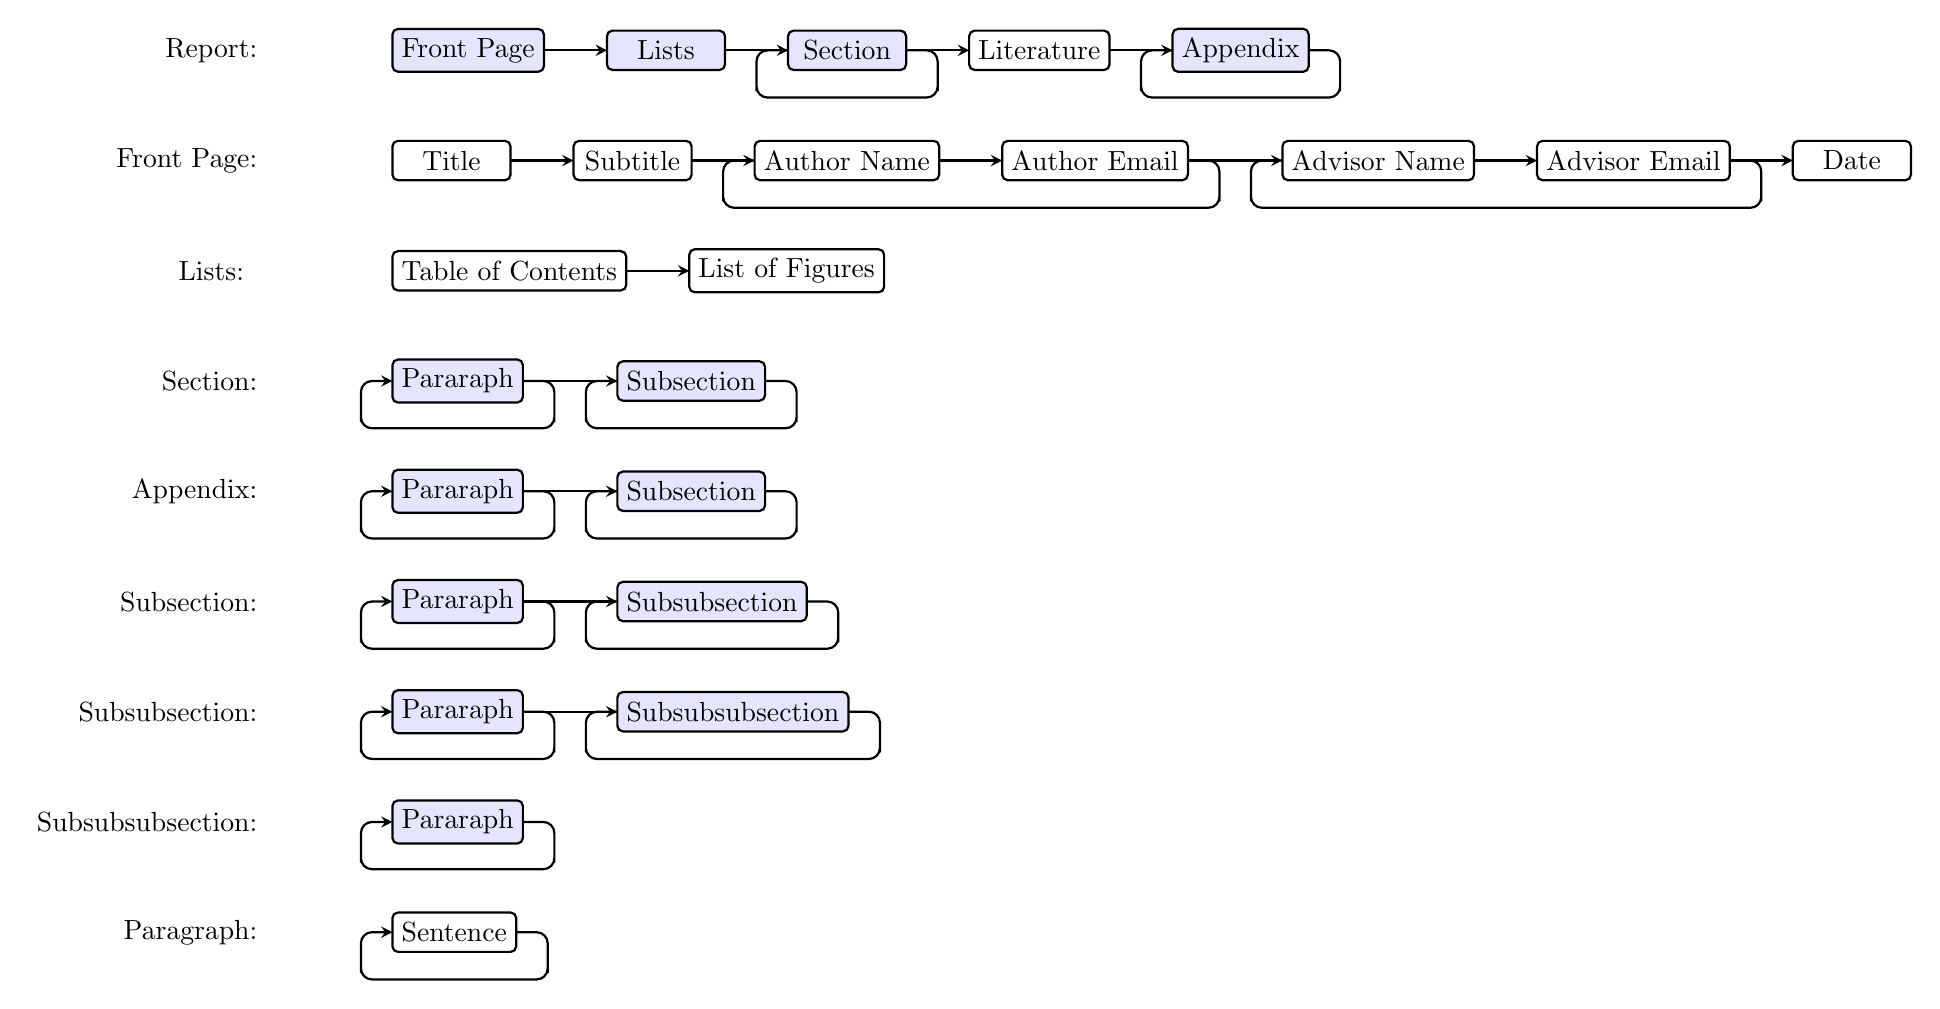
\begin{tikzpicture}[x=1cm, y=-1cm, node distance=0 cm,outer sep = 0pt]
          \newcommand{\textminheight}{5mm}
          \newcommand{\defminwidth}{14mm}
          \newcommand{\defxoffset}{-10mm}
          \newcommand{\spacing}{8mm}
          \newcommand{\loopheight}{6mm}
          
          \tikzstyle{node}=[
            draw,
            rectangle,
            rounded corners=2pt,
            minimum height=\textminheight,
            minimum width=1.5cm,
            fill=blue!10,
            anchor=west,
            thick
          ]
          \tikzstyle{nodet}=[
            draw,
            rectangle,
            rounded corners=2pt,
            minimum height=\textminheight,
            minimum width=1.5cm,
            fill=white!10,
            anchor=west,
            thick
          ]
          \tikzstyle{def}=[
            draw=none,
            minimum height=\textminheight,
            minimum width=\defminwidth,
            anchor=east,
          ]
          \tikzstyle{line} = [thick, rounded corners, draw=black]
          \tikzstyle{arrow} = [thick,->,>=stealth, draw=black]
          
          \coordinate (origo) at (1,1);
          \coordinate (oreport)           at ([xshift=0, yshift=0mm] origo);
          \coordinate (ofront)            at  ([xshift=0, yshift=-1*(\textminheight+\loopheight*1.5)] origo);
          \coordinate (olists)            at  ([xshift=0, yshift=-2*(\textminheight+\loopheight*1.5)] origo);
          \coordinate (osection)          at  ([xshift=0, yshift=-3*(\textminheight+\loopheight*1.5)] origo);
          \coordinate (oappendix)         at  ([xshift=0, yshift=-4*(\textminheight+\loopheight*1.5)] origo);
          \coordinate (osubsection)       at  ([xshift=0, yshift=-5*(\textminheight+\loopheight*1.5)] origo);
          \coordinate (osubsubsection)    at ([xshift=0, yshift=-6*(\textminheight+\loopheight*1.5)] origo);
          \coordinate (osubsubsubsection) at ([xshift=0, yshift=-7*(\textminheight+\loopheight*1.5)] origo);
          \coordinate (oparagraph)        at ([xshift=0, yshift=-8*(\textminheight+\loopheight*1.5)] origo);
          
          % report
          \node[def] (defreport) at ([xshift=\defxoffset] oreport) {Report:};
          \node[node] (report_front) at ([xshift=\defxoffset+\spacing*2] oreport) {Front Page};
          \node[node] (report_lists) at ([xshift=\spacing] report_front.east) {Lists};
          \node[node] (report_section) at ([xshift=\spacing] report_lists.east) {Section};
          \node[nodet] (report_lit) at ([xshift=\spacing] report_section.east) {Literature};
          \node[node] (report_appendix) at ([xshift=\spacing] report_lit.east) {Appendix};
          \draw[arrow] (report_front) -- (report_lists);
          \draw[arrow] (report_lists) -- (report_section);
          \draw[arrow] (report_section) -- (report_lit);
          \draw[arrow] (report_lit) -- (report_appendix);
          \draw[line] (report_section.east) -- ++(\spacing/2,0em) |- ++(0em,-\loopheight) |- ([xshift=-\spacing/2, yshift=-\loopheight] report_section.west) -| ([xshift=-\spacing/2] report_section.west) -- (report_section.west);
          \draw[line] (report_appendix.east) -- ++(\spacing/2,0em) |- ++(0em,-\loopheight) |- ([xshift=-\spacing/2, yshift=-\loopheight] report_appendix.west) -| ([xshift=-\spacing/2] report_appendix.west) -- (report_appendix.west);
          
          % front page
          \node[def] (deffront) at ([xshift=\defxoffset] ofront) {Front Page:};
          \node[nodet] (front_title) at ([xshift=\defxoffset+\spacing*2] ofront) {Title};
          \node[nodet] (front_subtitle) at ([xshift=\spacing] front_title.east) {Subtitle};
          \node[nodet] (front_author_n) at ([xshift=\spacing] front_subtitle.east) {Author Name};
          \node[nodet] (front_author_e) at ([xshift=\spacing] front_author_n.east) {Author Email};
          \node[nodet] (front_advisor_n) at ([xshift=\spacing*1.5] front_author_e.east) {Advisor Name};
          \node[nodet] (front_advisor_e) at ([xshift=\spacing] front_advisor_n.east) {Advisor Email};
          \node[nodet] (front_date) at ([xshift=\spacing] front_advisor_e.east) {Date};
          \draw[arrow] (front_title) -- (front_subtitle);
          \draw[arrow] (front_subtitle) -- (front_author_n);
          \draw[arrow] (front_author_n) -- (front_author_e);
          \draw[arrow] (front_author_e) -- (front_advisor_n);
          \draw[arrow] (front_advisor_n) -- (front_advisor_e);
          \draw[arrow] (front_advisor_e) -- (front_date);
          \draw[line] (front_author_e.east) -- ++(\spacing/2,0em) |- ++(0em,-\loopheight) |- ([xshift=-\spacing/2, yshift=-\loopheight] front_author_n.west) -| ([xshift=-\spacing/2] front_author_n.west) -- (front_author_n.west);
          \draw[line] (front_advisor_e.east) -- ++(\spacing/2,0em) |- ++(0em,-\loopheight) |- ([xshift=-\spacing/2, yshift=-\loopheight] front_advisor_n.west) -| ([xshift=-\spacing/2] front_advisor_n.west) -- (front_advisor_n.west);
          
          % lists
          \node[def] (deflists) at ([xshift=\defxoffset] olists) {Lists:};
          \node[nodet] (lists_toc) at ([xshift=\defxoffset+\spacing*2] olists) {Table of Contents};
          \node[nodet] (lists_lof) at ([xshift=\spacing] lists_toc.east) {List of Figures};
          \draw[arrow] (lists_toc) -- (lists_lof);
          
          % section
          \node[def] (defsection) at ([xshift=\defxoffset] osection) {Section:};
          \node[node] (section_paragraph) at ([xshift=\defxoffset+\spacing*2] osection) {Pararaph};
          \node[node] (section_subsection) at ([xshift=\spacing*1.5] section_paragraph.east) {Subsection};
          \draw[arrow] (section_paragraph) -- (section_subsection);
          \draw[arrow, rounded corners] (section_paragraph.east) -- ++(\spacing/2,0em) |- ++(0em,-\loopheight) |- ([xshift=-\spacing/2, yshift=-\loopheight] section_paragraph.west) -| ([xshift=-\spacing/2] section_paragraph.west) -- (section_paragraph.west);
          \draw[line] (section_subsection.east) -- ++(\spacing/2,0em) |- ++(0em,-\loopheight) |- ([xshift=-\spacing/2, yshift=-\loopheight] section_subsection.west) -| ([xshift=-\spacing/2] section_subsection.west) -- (section_subsection.west);
          
          % appendix
          \node[def] (defappendix) at ([xshift=\defxoffset] oappendix) {Appendix:};
          \node[node] (appendix_paragraph) at ([xshift=\defxoffset+\spacing*2] oappendix) {Pararaph};
          \node[node] (appendix_subsection) at ([xshift=\spacing*1.5] appendix_paragraph.east) {Subsection};
          \draw[arrow] (appendix_paragraph) -- (appendix_subsection);
          \draw[arrow, rounded corners] (appendix_paragraph.east) -- ++(\spacing/2,0em) |- ++(0em,-\loopheight) |- ([xshift=-\spacing/2, yshift=-\loopheight] appendix_paragraph.west) -| ([xshift=-\spacing/2] appendix_paragraph.west) -- (appendix_paragraph.west);
          \draw[line] (appendix_subsection.east) -- ++(\spacing/2,0em) |- ++(0em,-\loopheight) |- ([xshift=-\spacing/2, yshift=-\loopheight] appendix_subsection.west) -| ([xshift=-\spacing/2] appendix_subsection.west) -- (appendix_subsection.west);
          
          % subsection
          \node[def] (defsubsection) at ([xshift=\defxoffset] osubsection) {Subsection:};
          \node[node] (subsection_paragraph) at ([xshift=\defxoffset+\spacing*2] osubsection) {Pararaph};
          \node[node] (subsection_subsubsection) at ([xshift=\spacing*1.5] subsection_paragraph.east) {Subsubsection};
          \draw[arrow] (subsection_paragraph) -- (subsection_subsubsection);
          \draw[arrow, rounded corners] (subsection_paragraph.east) -- ++(\spacing/2,0em) |- ++(0em,-\loopheight) |- ([xshift=-\spacing/2, yshift=-\loopheight] subsection_paragraph.west) -| ([xshift=-\spacing/2] subsection_paragraph.west) -- (subsection_paragraph.west);
          \draw[line] (subsection_subsubsection.east) -- ++(\spacing/2,0em) |- ++(0em,-\loopheight) |- ([xshift=-\spacing/2, yshift=-\loopheight] subsection_subsubsection.west) -| ([xshift=-\spacing/2] subsection_subsubsection.west) -- (subsection_subsubsection.west);
          
          % subsubsection
          \node[def] (defsubsubsection) at ([xshift=\defxoffset] osubsubsection) {Subsubsection:};
          \node[node] (subsubsection_paragraph) at ([xshift=\defxoffset+\spacing*2] osubsubsection) {Pararaph};
          \node[node] (subsubsection_subsubsubsection) at ([xshift=\spacing*1.5] subsubsection_paragraph.east) {Subsubsubsection};
          \draw[arrow] (subsubsection_paragraph) -- (subsubsection_subsubsubsection);
          \draw[arrow, rounded corners] (subsubsection_paragraph.east) -- ++(\spacing/2,0em) |- ++(0em,-\loopheight) |- ([xshift=-\spacing/2, yshift=-\loopheight] subsubsection_paragraph.west) -| ([xshift=-\spacing/2] subsubsection_paragraph.west) -- (subsubsection_paragraph.west);
          \draw[line] (subsubsection_subsubsubsection.east) -- ++(\spacing/2,0em) |- ++(0em,-\loopheight) |- ([xshift=-\spacing/2, yshift=-\loopheight] subsubsection_subsubsubsection.west) -| ([xshift=-\spacing/2] subsubsection_subsubsubsection.west) -- (subsubsection_subsubsubsection.west);
          
          % subsubsubsection
          \node[def] (defsubsubsubsection) at ([xshift=\defxoffset] osubsubsubsection) {Subsubsubsection:};
          \node[node] (subsubsubsection_paragraph) at ([xshift=\defxoffset+\spacing*2] osubsubsubsection) {Pararaph};
          \draw[arrow, rounded corners] (subsubsubsection_paragraph.east) -- ++(\spacing/2,0em) |- ++(0em,-\loopheight) |- ([xshift=-\spacing/2, yshift=-\loopheight] subsubsubsection_paragraph.west) -| ([xshift=-\spacing/2] subsubsubsection_paragraph.west) -- (subsubsubsection_paragraph.west);
          
          % paragraph
          \node[def] (defparagraph) at ([xshift=\defxoffset] oparagraph) {Paragraph:};
          \node[nodet] (paragraph_sentence) at ([xshift=\defxoffset+\spacing*2] oparagraph) {Sentence};
          \draw[arrow, rounded corners] (paragraph_sentence.east) -- ++(\spacing/2,0em) |- ++(0em,-\loopheight) |- ([xshift=-\spacing/2, yshift=-\loopheight] paragraph_sentence.west) -| ([xshift=-\spacing/2] paragraph_sentence.west) -- (paragraph_sentence.west);
        \end{tikzpicture}
      }
    \end{adjustbox}
  \caption{\label{fig:firststeps:process:bnf} Railroad BNF of a typical report structure.}
\end{figure}

% differences in opinion
But how do you come up with that tree structure; the \textsl{right} tree structure? People tend to prefer one of two strategies, and despise the other. I have seen both work for people who chose it of their own free will.

% first strat
The first strategy is to first get something (anything, really) down "on paper", and then iterate and keep on iterating until the end result is good. I am not a fan of this approach. Generally, it requires a lot of writing experience to succeed, the overhead of repeated iterations is high, and the iterations usually end up being cut short before a good result has been reached.

% second strat
The second strategy is to go top-down by growing the tree from the root. Only after understanding the final structure of a node (at a single level of depth) are you allowed to dig into a child node. Note that this allows you to go deep in some parts of the report while having little understanding of others.

% second strat: mindset
That implies a process of considering the topic of the node and all that came before it, and deciding:
\begin{enumerate}
  \item Which key points have to be covered?
  \item Which pseudo points are needed to support these?
  \item What is the best way of serializing the coverage of all of these points?
  \item How can that sequence be broken down into themes?
\end{enumerate}
These themes are your subsections. Often it makes sense to consider naming conventions that transcends a single subtree to bring some consistency to the report.

% second strat: tool
Large reports can become hard to navigate and conclusions on the exact contents of som subsection may escape memory. One way of dealing with this is to write down pre and post conditions for individual (sub*)sections. This works particularly well in \LaTeX\ where you have comments:

\begin{minted}[breaklines]{latex}
\subsection{Publish Subscribe Substrates}
\label{sec:analysis:transport:pubsub}
% pre: It has been established that a transport is needed for moving streaming data from backend to front-end at a rate of 10-20Hz. Parameters for evaluation: [latency, throughput, robustness, inspection].
% post: A clear definition of the pros and cons of using pubsub for this purpose.
\end{minted}

\section{Working Document}

It is a good practice in a project to quickly establish a working report document. That gives you a natural area to drop notes about your design choices (so that you can later remember why you did things the way you ended up doing them) and have a low bar for writing on your report should you suddenly feel inspired. You can organically structure the report as your perception of its shape matures, and -- if frequently visited -- it will keep your mind fixed on which details matter for the end-goal of producing the report handin.

This document represents a dissertation. In the beginning of it you are likely to have a central thesis, or maybe a number of theses that you wish to explore. The starting point is what you came up with in your project description (see section \ref{sec:projectdesc}). I recommend filling out the contents of each section as you go through the corresponding phases of the project. That way the details are still sharp in your mind, it is easy to make sure that you don't miss anything, and you don't end up with a whole lot of report work at the end.

\section{Report Structure}

The following is a good starting point for the structure of most reports.

\begin{enumerate}
  \descitem{Introduction} 
    \begin{enumerate}[label*=\arabic*.]
      \descitem{Problem}
      \descitem{Approach}
    \end{enumerate}
  \descitem{Process}
  \descitem{Related Work}
  \descitem{Analysis}
  \descitem{Design}
  \descitem{Evaluation}
  \descitem{Discussion}
  \descitem{Future Work}
  \descitem{Hindsight}
  \descitem{Conclusion}
  \descitem{Literature}
  \descitem{Appendix}
\end{enumerate}

%%%%%%%%%%%%%%%%%%%%%%%%%%%%%%%%%%%%%%%%%%%%%%%%%%%%%%%%%%%%%%%%%%%%%%%%%%%%%%%%
%%%%%%%%%%%%%%%%%%%%%%%%%%%%%%%%%%%%%%%%%%%%%%%%%%%%%%%%%%%%% The Art of Writing
\chapter{The Art of Writing}

\section{Commandments}

\begin{enumerate}
  \descitem{Make the Effort}
    As with pretty much else in life, if you want to excel at writing you need to put in significant amounts of focused work and active considerations about the nature of what makes a text good. Take pride in your work.
  \descitem{It Has to Make Sense}
    Above all else, what you do (and write) has to make sense. This should be your guiding light throughout the entire project. Much can be excused as long as the it is done for the right reasons. While this is used to balance learning objectives according to the individual project, in cannot completely remove a learning objective.
  \descitem{Give and Take Credit}
    In order to evaluate the contribution of a text it is necessary to know which parts the author has been responsible for contributing. If some insight, term or similar is original, then credit should be given to the author. If not, then credit should be given to the original authors (e.g., through a citation) and credit should be given to the author for citing them. It is bad practice to leave credit unclear, and it erodes overall confidence in the text itself. Therefore, always make sure that you give credit where it is needed, and take credit where you can.
  \descitem{Best Practices are Fallacies}
    While it is a good practice to explore best practices, real projects never seem to be quite that simple. Best practices are based on typical situations, and it is thus a good practice to be critical towards them. You will likely have to violate one or two of them.
  \descitem{Do not Underestimate Experimental Evaluation}
    When working on something of experimental nature it is hard to assess the time to completion. Before beginning the work it is harder. Does all the needed experimental tooling already exists, or do you need to construct parts of it yourself? How many repetitions are necessary to get trustworthy results? How much time is needed to conduct the experiments? Which kinds of post processing of results are needed to reach the relevant insights?
    However long you think it is going to take, it is going to take longer. In part because things are going to go wrong, and you might realize that your design needs to change. For that to even be a possibility, you need to start experimental work early. A good rule of thumb is to take the time you expect it to take, and multiply it by $\pi$.
  \descitem{Respect your Audience}
    You are writing a report because you expect someone to read it. Knowing who that someone is is key to understanding what is necessary in order to convey your subject. You can expect your reader to have an IT-related background and at least an MSc. Also, you should expect the reader to print your report on A4 paper. A consequence of this is that you cannot rely on the reader zooming in to read certain parts of a figure.
  \descitem{One sentence One message}
    Rarely is anything achieved by having a single sentence deliver more than a single message. Often, readability is affected negatively. A sequence of short messages, each progressing the narrative towards a point is a simple way of ensuring a concise and readable language. It takes considerable effort to shoehorn multiple messages into a single sentence without negatively affecting readability.
  \descitem{A Text Should Be Self-Contained}
    A text (e.g., a paragraph) may refer to other resources like sections, citations, appendices or floats (figures and tables), but the reader should not need to follow any of these to read the text. So, when referring to a figure make sure to highlight what you would get out of looking at it. The reader then has a \textsl{choice} of looking at the figure. In much the same way, when looking at the figure the reader should not have to look for a reference in the text for that figure in order to understand how to read it. Instead these details should be covered by a legend or the figures label.
  \descitem{The Specific-Generic Spectrum} % Can we make this statement more specific to a degree where it is as wide as possible without becoming untrue for some cases?
    Most statements has (at least one) inherent specificity. That is, what it expresses fits on a scale from specific to generic. If a statement is too generic then part of it is untrue. That is obviously problematic. If a statement is too specific then it doesn't express the full gamut of the underlying mechanics. That is less-obviously problematic. Perhaps it doesn't need to be covered to make your point, but it is makes it unclear whether you actually understand those implications. So, make every statement specific to a degree where it is as wide as possible without becoming untrue for any case.
  \descitem{Make the Argument Explicit}
    When providing an argument, do not rely on the reader to fold out steps that you consider implicit. The reader may have other standards for what is implicit, or have a different cultural background where those steps are not obvious. Also, this is an opportunity to show that you can construct a line of reasoning, and that opportunity should be grabbed.
  \descitem{Remember the Context}
    Everything communicated is expressed in some context. Key aspects of this context are necessary to correctly decipher the communication. Be aware of these aspects and make sure that they are shared with the reader. For instance, the word \quoted{technical} can be rooted in software, but could also be legal or mechanical. I assume that people from legal also refer to the technical aspects, but have a fairly different interpretation of what that means.
\end{enumerate}

\section{Pieces}

\subsection{Definitions}

\section{Questions}

\begin{itemize}
  \descitem{From a scientific point of view -- why does it matter?}
\end{itemize}

\section{Anti-Patterns}

\subsection{Use-Before-Definition}

\subsection{Overuse of Utilize}

\subsection{Reason-Therefore-Reason}

% Because of the "Therefore" you already have a reason and that reason will appear -- to the reader -- to be in conflict with what comes after the "as" of the last sentence.

\subsection{Sentence Repetition}

% First introducing a general statement, and then providing two examples

\subsection{Two Paragraphs for Single Purpose}

% This paragraph serves exactly the same purpose as the previous one, and as the saying goes: There can be only one!

\subsection{Should Without a Question}

% Leading with a "should" tells the reader that you are asking a question. If you flip it around (i.e., research should) makes a concluding statement.

\subsection{Triple Linespacing}

Increased the line spacing is something used by public school teachers to write grammar notes on print. You are expected to write grammatically correct text when you reach the university level so we don't do that. Please stick to a reasonable line spacing. In reality, increasing the line spacing makes the report appear \textsl{thin}.

%%%%%%%%%%%%%%%%%%%%%%%%%%%%%%%%%%%%%%%%%%%%%%%%%%%%%%%%%%%%%%%%%%%%%%%%%%%%%%%%
%%%%%%%%%%%%%%%%%%%%%%%%%%%%%%%%%%%%%%%%%%%%%%%%%%%%%%%%%%%%%%%%%%% Introduction
\chapter{Introduction}

%%%%%%%%%%%%%%%%%%%%%%%%%%%%%%%%%%%%%%%%%%%%%%%%%%%%%%%%%%%%%%%%%%%%%%%%%%%%%%%%
%%%%%%%%%%%%%%%%%%%%%%%%%%%%%%%%%%%%%%%%%%%%%%%%%%%%%%%%%%%%%% Literature Review
\chapter{Literature Review}

% purpose

\section{Goals}

\section{Building Blocks}

\section{Documentation}

\section{Presentation}

%%%%%%%%%%%%%%%%%%%%%%%%%%%%%%%%%%%%%%%%%%%%%%%%%%%%%%%%%%%%%%%%%%%%%%%%%%%%%%%%
%%%%%%%%%%%%%%%%%%%%%%%%%%%%%%%%%%%%%%%%%%%%%%%%%%%%%%%%%%%%%%%%%%% Requirements
\chapter{Requirements}

\section{Testability}

I often come across requirements like \quoted{The system should be responsive}. On the surface it appears fine, even sane. However, it is not testable. There is no agreement as to what it means for a system to be \quoted{responsive}. It is what is sometimes referred to as a \quoted{bad requirement}.

Usually, we have requirements because we need something to evaluate a resulting system against. For this purpose, the above mentioned requirement is useless, and it is your problem not spotting it in due time.

Sometimes this kind of problematic requirement can be \quoted{leveled up}. In this particular case it might be clear that the \quoted{responsiveness} property relates to the users of the system. That, in and of itself, doesn't help us much, but it does give us something to work with: We could construct a system that exposes users to varying response times and ask them to rank different runs as either \quoted{responsive} or \quoted{not responsive}. That way we can \textsl{quantify} what it means to be responsive in this context.

\textbf{Note:} This would be part of the requirement analysis, as you will need a good understanding of the requirements before starting on the design.

%%%%%%%%%%%%%%%%%%%%%%%%%%%%%%%%%%%%%%%%%%%%%%%%%%%%%%%%%%%%%%%%%%%%%%%%%%%%%%%%
%%%%%%%%%%%%%%%%%%%%%%%%%%%%%%%%%%%%%%%%%%%%%%%%%%%%%%%%%%%%%%%%%%%%%%% Analysis
\chapter{Analysis}

%%%%%%%%%%%%%%%%%%%%%%%%%%%%%%%%%%%%%%%%%%%%%%%%%%%%%%%%%%%%%%%%%%%%%%%%%%%%%%%%
%%%%%%%%%%%%%%%%%%%%%%%%%%%%%%%%%%%%%%%%%%%%%%%%%%%%%%%%%%%%%%%%%%%%%%%%% Design
\chapter{Design}

%%%%%%%%%%%%%%%%%%%%%%%%%%%%%%%%%%%%%%%%%%%%%%%%%%%%%%%%%%%%%%%%%%%%%%%%%%%%%%%%
%%%%%%%%%%%%%%%%%%%%%%%%%%%%%%%%%%%%%%%%%%%%%%%%%%%%%%%%%%%%%%%%% Implementation
\chapter{Implementation}

%%%%%%%%%%%%%%%%%%%%%%%%%%%%%%%%%%%%%%%%%%%%%%%%%%%%%%%%%%%%%%%%%%%%%%%%%%%%%%%%
%%%%%%%%%%%%%%%%%%%%%%%%%%%%%%%%%%%%%%%%%%%%%%%%%%%%%%%%%%%%%%%%%%%%% Evaluation
\chapter{Evaluation}

% intro:
When you have constructed your system, you have certainly achieved something. But at that point we know very little about \textsl{what} you have achieved. Does it work correctly? How well does it meet the requirements? To be able to make claims in these regards, you need an evaluation. What and how you need to evaluate depends on which kinds of claims you wish to make. At the end of the day the claims supported by your evaluation will define the success of the system. From a report perspective, that is.

% TODO: needs a rewrite:
My recommendation is for you to think the evaluation into the design so that you end up designing for evaluation. One benefit of that would be that your mental model of the evaluation process evolves along with the project. Another would be that that you end up having natural points for instrumentation in the codebase that gives you exactly the kind of access that you need for your *ideal* evaluation.

\section{Criteria}

\subsection{Correctness}

\subsection{Usability}

\subsection{Performance}

\subsection{Availability}

\subsection{Scalability}

\section{Methods}

% argument: what is

\subsection{Textual Argument}

\subsection{Performance Evaluation}

\subsection{User Test}

\section{Process}

Go through the requirements; one at a time. Determine the best way of evaluating this particular requirement. 

\begin{figure}[tbp]
  contents
  \caption{Method suitability for various criteria.}
\end{figure}

\section{Presentation}

%%%%%%%%%%%%%%%%%%%%%%%%%%%%%%%%%%%%%%%%%%%%%%%%%%%%%%%%%%%%%%%%%%%%%%%%%%%%%%%%
%%%%%%%%%%%%%%%%%%%%%%%%%%%%%%%%%%%%%%%%%%%%%%%%%%%%%%%%%%%%%%%%%%%%% Discussion
\chapter{Discussion}

%%%%%%%%%%%%%%%%%%%%%%%%%%%%%%%%%%%%%%%%%%%%%%%%%%%%%%%%%%%%%%%%%%%%%%%%%%%%%%%%
%%%%%%%%%%%%%%%%%%%%%%%%%%%%%%%%%%%%%%%%%%%%%%%%%%%%%%%%%%%%%%%%%%%% Future Work
\chapter{Future Work}

%%%%%%%%%%%%%%%%%%%%%%%%%%%%%%%%%%%%%%%%%%%%%%%%%%%%%%%%%%%%%%%%%%%%%%%%%%%%%%%%
%%%%%%%%%%%%%%%%%%%%%%%%%%%%%%%%%%%%%%%%%%%%%%%%%%%%%%%%%%%%%%%%%%%%% Conclusion
\chapter{Conclusion}

%%%%%%%%%%%%%%%%%%%%%%%%%%%%%%%%%%%%%%%%%%%%%%%%%%%%%%%%%%%%%%%%%%%%%%%%%%%%%%%%
%%%%%%%%%%%%%%%%%%%%%%%%%%%%%%%%%%%%%%%%%%%%%%%%%%%%%%%%%%%%%%%%%%%% Post Handin
\chapter{Post Handin}

After handing in, and having licked your wounds, it's time to start considering the oral defense of the project.

% point of the defense: learning objectives

\section{Presentation Structure}

The following is a good starting point for the presentation structure:
\begin{enumerate}
  \descitem{Front Page} Including the title, your names and email, advisors name and email\textcolor{teal}{[1 slide]}.
  \descitem{Context} The information necessary for understanding the following slides\textcolor{teal}{[0-1 slide]}.
  \descitem{Problem} Problem statement\textcolor{teal}{[1 slide]}.
  \descitem{Approach} High-level strategy for solving the problem\textcolor{teal}{[1 slide]}.
  \descitem{Analysis} Analysis of the problem domain\textcolor{teal}{[1 slide per subject]}.
  \descitem{Design} Description of the resulting design\textcolor{teal}{[1+ slide per subject]}.
  \descitem{Implementation} Any unique implementation details\textcolor{teal}{[1 slide per detail, could be 0]}.
  \descitem{Demo} Switch to demo if fitting for project\textcolor{teal}{[1 slide]}.
  \descitem{Evaluation} For each area that needed to be evaluated; (i) what needed to be evaluated? (ii) how did you evaluate it? and (iii) what was the result of the evaluation?\textcolor{teal}{[1-2 slides per area]}.
  \descitem{Future Work} In which directions would it make sense to take this?\textcolor{teal}{[0-1 slide]}.
  \descitem{Conclusion} Summary of conclusions \textcolor{teal}{[1 slide]}.
\end{enumerate}

% style: don't read aloud from the slides, bulletpoints can work as a starting point, no stock photos (they need to add value), use figures and tables from the report, if you can't find the figures you need in the report chances are that it is missing them
Figures make great partners when you explain something. It allows you to point at the thing you are explaining and functions as visual anchor should you temporarily look the train of thought. Your report should already have most or all of the figures you are going to need. If it doesn't, then you should consider why that is? But sometimes a figure is not the right companion. Bulletpoints or enumerations might be. They allow you to place keywords in your field of vision. Generally speaking, the more hints you can give yourself and the audience the better. However, you shouldn't take this to the extreme: The ability to read a text aloud won't impress censor.

\section{Defense}

The allocated time for the defense can be seen in figure \ref{fig:defense:time}\footnote{Please note that this may not be up to date.}.

\begin{figure}
  \centering
  \scalebox{0.93}{
  \begin{tabular}{llccrr}
    \emph{Education} & \emph{Level} & \emph{ECTS} & \emph{Group} & \centering \emph{Total} & \emph{Presentation} \\
     & & \emph{[ECTS]} & \emph{Size} & \emph{Time [min]} & \emph{Time [min]} \\
    Software Engineering & BSc & 15 & 1 & 30 & 10-12 \\
    Software Engineering & BSc & 15 & 2 & 60 & 15-20 \\
    Software Engineering & BSc & 15 & 3 & 90 & 20-25 \\
    Software Engineering & MSc & 30 or 60 & 1 & 60 & 15-20 \\
    Software Engineering & MSc & 30 or 60 & 2 & 120 & 30-40 \\
    Software Engineering & MSc & 30 or 60 & 3 & 180 & 40-60 \\
    Software Technology & BSc+ & 30 & 1 & 45 & 12-20 \\
    Software Technology & BSc+ & 30 & 2 & 90 & 20-25 \\
    Software Technology & BSc+ & 30 & 3 & 135 & 30-45 \\
  \end{tabular}
  }
  \caption{\label{fig:defense:time} Time allocations for various defenses.}
\end{figure}

% defense sequence: overview, presentation split, indicators for who did what

% language:
You are always allowed to conduct the presentation in English. If censor knows Danish, then Danish becomes an option as well. My recommendation is that the slides are written in English either way. The language for the presentation and the language for the following individual defense are not required to be the same. You decide.

% be critical, admit mistakes, explain them, describe what you have learnt and how to avoid it in the future
Few projects go according to plan, and mistakes are frequently made. There are not problems. Revisiting these situations, figuring out what the problem was and how you could have handled the situation better is actually a positive. It shows that you can be critical of your own work, and learn from your mistakes. As we know everybody makes mistakes. This provides the recipient with insights into how you deal with the.

\subsection{Presentation}

% distribution of time (between group members)
When presenting, be sure to distribute the presentation duties roughly evenly across all group members. It doesn't matter too much how large segments each member presents at a time, so try to find a natural balance. However, if no other indication of who did what is available, censor and advisor may try to glen this from the mapping from contents to group member.

% clarifying uncertainties
After the presentation, advisor and censor are likely to have e few questions to clarify uncertainties before progressing to the individual part of the exam.

\subsection{Questions}

% based on learning objectives: clear pass -> verify, middle -> can we pull up? (expectation high), bottom -> can we pull up (expectation low)?, within the given restrictions (e.g., time), => we are going to sample
Some questions will seek to clarify what have been done, and others will address the reasoning behind the choices. In general, we look at the learning objectives. If a learning objective is a clear pass then the goal is to verify that you did the job. If a learning objective is partially fulfilled then the goal is to see if the level of the student is higher than that of the report. The same goes for learning objectives which have not been fulfilled, but here the expectation is low. Because of the time restrictions the questions will represent an attempt to sample enough insights to land on a grade.

% code: may ask about code in report main, highly unlikely to ask about the rest of the code
During the examination we generally try to stay away from code. If there is something in the report main that sticks out it might warrant a follow up, and then it could potentially be taken all the way. In practice, that doesn't happen though.

\section{Evaluation}

% report perception: report grade, usually +-1 grade, maybe more, potentially+exceptionally all the way down
The report (likely) contains many pages and covers much information. You have spent a significant amount of time on it with few restrictions. Censor and examiner has spent a great deal of time reading it. Compared to that, the defense represents a small amount of time. Coming into the defense, both censor and examiner will have a rough idea of the level of the report, and it is generally -- in the brief time allotted -- hard to sway that perception. Typically, the end results will fall within $\pm 1$ grade step of that initial impression. It does happen that the final grade is shifted more, but it is rare. In exceptional cases (e.g., if it is discovered that someone hasn't participated), the grade could potentially go all the way down.

\end{document}
